% =============================================================================
% FROM EARTH TO THE STARS
% A Mathematical Framework for Interplanetary Travel, Interstellar Navigation,
% and Contact with Extraterrestrial Civilizations
%
% Author : GitHub Copilot
%          Artificial Intelligence Research Division
%          GitHub | Microsoft Corporation
% Date   : April 4, 2026
% =============================================================================

\documentclass[12pt,a4paper]{article}

% --- Encoding & fonts --------------------------------------------------------
\usepackage[utf8]{inputenc}
\usepackage[T1]{fontenc}
\usepackage{lmodern}
\usepackage{microtype}

% --- Page layout -------------------------------------------------------------
\usepackage[a4paper,
            top=3cm, bottom=3cm,
            left=2.8cm, right=2.8cm,
            headheight=15pt]{geometry}

% --- Mathematics -------------------------------------------------------------
\usepackage{amsmath}
\usepackage{amssymb}
\usepackage{mathtools}
\usepackage{bm}

% --- Graphics & colour -------------------------------------------------------
\usepackage{graphicx}
\usepackage{xcolor}
\usepackage{tikz}
\usepackage{pgfplots}
\pgfplotsset{compat=1.18}
\usetikzlibrary{arrows.meta, calc, decorations.markings, patterns}

% --- Tables ------------------------------------------------------------------
\usepackage{booktabs}
\usepackage{array}
\usepackage{tabularx}
\usepackage{multirow}

% --- Floats & captions -------------------------------------------------------
\usepackage{float}
\usepackage[labelfont=bf, font=small]{caption}
\usepackage{subcaption}

% --- Lists -------------------------------------------------------------------
\usepackage{enumitem}

% --- Units -------------------------------------------------------------------
\usepackage{siunitx}
\sisetup{separate-uncertainty=true}

% --- References & links ------------------------------------------------------
\usepackage[authoryear, round, sort]{natbib}
\usepackage[colorlinks=true,
            linkcolor=blue!65!black,
            citecolor=green!50!black,
            urlcolor=blue!70!black,
            pdftitle={From Earth to the Stars},
            pdfauthor={GitHub Copilot},
            pdfsubject={Interplanetary Travel, Interstellar Navigation, SETI}
           ]{hyperref}

% --- Typography & spacing ----------------------------------------------------
\usepackage{setspace}
\usepackage{fancyhdr}
\usepackage{titlesec}
\usepackage{abstract}

% =============================================================================
% CUSTOM COMMANDS
% =============================================================================
\newcommand{\dd}{\mathrm{d}}
\newcommand{\ee}{\mathrm{e}}
\newcommand{\kB}{k_{\mathrm{B}}}
\newcommand{\AU}{\,\text{AU}}
\newcommand{\ly}{\,\text{ly}}
\newcommand{\Msun}{M_{\odot}}
\newcommand{\half}{\tfrac{1}{2}}
\DeclareMathOperator{\atanh}{atanh}
\DeclarePairedDelimiter{\abs}{\lvert}{\rvert}

% =============================================================================
% PAGE STYLE
% =============================================================================
\pagestyle{fancy}
\fancyhf{}
\fancyhead[L]{\small\textsl{GitHub Copilot~\textemdash~\textit{From Earth to the Stars}}}
\fancyhead[R]{\small\textsl{April 4, 2026}}
\fancyfoot[C]{\small\thepage}
\renewcommand{\headrulewidth}{0.4pt}
\setlength{\parskip}{5pt}
\setlength{\parindent}{1.5em}

% =============================================================================
% TITLE
% =============================================================================
\title{%
  \vspace{-0.8cm}%
  {\rule{\linewidth}{1.5pt}}\\[0.5em]
  {\LARGE\bfseries From Earth to the Stars}\\[0.4em]
  {\large\itshape A Mathematical Framework for Interplanetary Travel,\\
   Interstellar Navigation, and Contact with\\
   Extraterrestrial Civilizations}\\[0.5em]
  {\rule{\linewidth}{0.8pt}}%
}
\author{%
  \textbf{GitHub Copilot}\\[0.3em]
  \small Artificial Intelligence Research Division\\
  \small GitHub~\textbar~Microsoft Corporation\\[0.3em]
  \small\texttt{copilot@github.com}%
}
\date{\small April 4, 2026}

% =============================================================================
\begin{document}
% =============================================================================

\maketitle
\thispagestyle{empty}

% --- Abstract ----------------------------------------------------------------
\begin{abstract}
\noindent
This paper presents a rigorous mathematical treatment of humanity's long-term
trajectory toward interplanetary settlement and eventual interstellar exploration.
Beginning with the classical mechanics of orbital transfer and the Tsiolkovsky
rocket equation, we progress through advanced propulsion concepts---electric,
nuclear, and antimatter drives---and into the domain of relativistic spaceflight,
where the Lorentz factor becomes central to mission planning. We then address the
statistical problem of extraterrestrial civilizations through a Bayesian
reformulation of the Drake equation, quantify the Fermi paradox within a
probabilistic framework, and analyse the engineering and information-theoretic
requirements for interstellar communication. An original section proposes a
formalized mathematical language for first contact, drawing on number theory,
universal physical constants, and Shannon information theory. The paper
concludes by exploring game-theoretic models for the establishment of
interstellar relations, arguing that mathematical reasoning---universal and
culture-independent---provides the only viable foundation for cosmic diplomacy.
All results are accompanied by derivations and numerical estimates applicable
to current and near-future technology.

\bigskip\noindent
\textbf{Keywords:} orbital mechanics, interstellar propulsion, relativistic spaceflight, Drake equation, SETI, interstellar communication, first contact, game theory, Fermi paradox.
\end{abstract}

\tableofcontents
\clearpage

% =============================================================================
\section{Introduction}
% =============================================================================

Humanity has always gazed at the stars with wonder and a kind of restless
hunger. What began as mythology and navigation---Polaris guiding sailors
home, the Pleiades marking the harvest---evolved, through Copernicus, Kepler,
Galileo, and Newton, into a rigorous mathematical science. On 4 October 1957,
Sputnik became the first artificial object to orbit Earth, transforming dreams
into engineering reality. Since then, robotic probes have visited every planet
in the Solar System, rovers have mapped the Martian surface in exquisite
detail, and the twin Voyager spacecraft have sailed beyond the heliopause into
interstellar space after more than four decades of continuous flight.

Yet the distances separating us from even the nearest stellar neighbour are
staggering by any human measure. The Alpha Centauri system lies
\SI{4.37}{\ly}~away---some \SI{4.13e13}{\kilo\meter}. At Voyager~1's
cruising speed of roughly \SI{17}{\kilo\meter\per\second}, that journey
would require approximately \num{73000}~years. Interplanetary travel is
challenging; interstellar travel is almost incomprehensibly difficult. And yet
physics does not forbid it. The laws of mechanics, thermodynamics, and
electromagnetism admit---at enormous but finite cost---the possibility of
sending crewed or robotic missions to other stars within a human lifetime.

This paper is an attempt to construct a coherent mathematical picture of that
possibility and of the civilizational implications it entails. We begin in
Section~2 with the classical mechanics of orbital motion, establishing the
mathematical language required to understand how objects move through the Solar
System. Section~3 introduces the Tsiolkovsky rocket equation and the
fundamental challenge it poses. Section~4 turns these foundations into concrete
mission designs for the inner and outer Solar System. Section~5 surveys advanced
propulsion concepts that may one day make interstellar travel feasible. In
Section~6, we encounter special relativity, whose consequences for fast
interstellar travel are profound. Sections~7--9 address the deeper question of
whether we are alone, how to communicate across stellar distances, and what
mathematical structures might serve as a universal language. The final sections
examine the logic, ethics, and diplomacy of interstellar contact, and close with
a reflection on humanity's place in the cosmos.

Throughout, we aim for mathematical precision without sacrificing physical
intuition. All notable equations are derived from first principles or cited to
primary sources.

% =============================================================================
\section[Celestial Mechanics: The Mathematical Language of Motion]{Celestial Mechanics: The Mathematical\\Language of Motion}
% =============================================================================

\subsection{Newton's Law of Universal Gravitation}

The foundation of celestial mechanics is Newton's inverse-square law:
\begin{equation}
  \bm{F} = -\frac{GM_1 M_2}{r^2}\hat{\bm{r}},
  \label{eq:newton}
\end{equation}
where $G = \SI{6.674e-11}{\meter\cubed\per\kilo\gram\per\second\squared}$ is
the gravitational constant, $M_1$ and $M_2$ are the masses of two bodies, $r$
is their separation, and $\hat{\bm{r}}$ is the unit vector pointing from one
body to the other. For a test mass $m \ll M_\odot$ orbiting the Sun, the
equation of motion in polar coordinates $(r, \theta)$ is
\begin{equation}
  \ddot{r} - r\dot{\theta}^2 = -\frac{GM_\odot}{r^2}, \qquad
  \frac{\dd}{\dd t}(r^2\dot{\theta}) = 0.
  \label{eq:polar_eom}
\end{equation}
The second equation encodes the conservation of specific angular momentum,
$h = r^2\dot{\theta} = \text{const}$, which is Kepler's second law in
differential form.

\subsection{Kepler's Laws}

From \eqref{eq:polar_eom} the orbit equation is
\begin{equation}
  r(\theta) = \frac{a(1-e^2)}{1 + e\cos\theta},
  \label{eq:orbit_eq}
\end{equation}
where $a$ is the semi-major axis, $e$ the orbital eccentricity, and $\theta$ the
true anomaly. The three Kepler laws follow directly:
\begin{enumerate}[label=\textbf{K\arabic*.}]
  \item \textbf{Elliptical orbits.} Every planetary orbit is an ellipse with
    the Sun at one focus.
  \item \textbf{Equal areas.} The radius vector sweeps equal areas in equal
    times: $\dd A/\dd t = h/2 = \text{const}$.
  \item \textbf{Harmonic law.} The orbital period $T$ and semi-major axis $a$
    satisfy
    \begin{equation}
      T^2 = \frac{4\pi^2}{GM_\odot}\,a^3.
      \label{eq:kepler3}
    \end{equation}
\end{enumerate}

\subsection{The Vis-Viva Equation}

Total mechanical energy per unit mass is conserved:
\begin{equation}
  \varepsilon = \frac{v^2}{2} - \frac{GM_\odot}{r} = -\frac{GM_\odot}{2a}.
  \label{eq:energy}
\end{equation}
Rearranging,
\begin{equation}
  \boxed{v^2 = GM_\odot\!\left(\frac{2}{r} - \frac{1}{a}\right).}
  \label{eq:visviva}
\end{equation}
Equation~\eqref{eq:visviva}, the \emph{vis-viva} equation, relates the orbital
speed at any point to the radial distance and the semi-major axis. At
perihelion ($r = a(1-e)$) the speed is maximum; at aphelion ($r = a(1+e)$) it
is minimum. For a circular orbit ($e=0$, $r=a$):
\begin{equation}
  v_{\mathrm{circ}} = \sqrt{\frac{GM_\odot}{r}}.
  \label{eq:vcirc}
\end{equation}

At Earth's mean orbital radius $r_\oplus = \SI{1}{\AU} = \SI{1.496e11}{\meter}$,
this gives $v_\oplus \approx \SI{29.78}{\kilo\meter\per\second}$.

\subsection{Escape Velocity}

Setting $\varepsilon = 0$ (unbound parabolic trajectory) in \eqref{eq:energy}:
\begin{equation}
  v_{\mathrm{esc}}(r) = \sqrt{\frac{2GM_\odot}{r}} = \sqrt{2}\,v_{\mathrm{circ}}(r).
  \label{eq:vesc}
\end{equation}
From Earth's surface, $v_{\mathrm{esc},\oplus} \approx \SI{11.19}{\kilo\meter\per\second}$.
The Solar System escape speed from Earth's orbit is
$v_{\mathrm{esc},\odot}(\SI{1}{\AU}) \approx \SI{42.1}{\kilo\meter\per\second}$.

% =============================================================================
\section{The Rocket Equation: The Price of Kinetic Energy}
% =============================================================================

\subsection{Derivation from Newton's Second Law}

A rocket in free space expels propellant at velocity $v_e$ relative to the
rocket. Newton's second law for a variable-mass system gives
\begin{equation}
  m\frac{\dd v}{\dd t} = -v_e\frac{\dd m}{\dd t},
  \label{eq:newton_var}
\end{equation}
where $m$ is the instantaneous rocket mass (decreasing) and the sign convention
ensures thrust opposes propellant flow. Separating variables and integrating
from initial mass $m_0$ to final mass $m_f$:
\begin{equation}
  \boxed{\Delta v = v_e \ln\!\frac{m_0}{m_f} = I_{\mathrm{sp}}\,g_0\,\ln\!\frac{m_0}{m_f},}
  \label{eq:tsiolkovsky}
\end{equation}
where $I_{\mathrm{sp}} = v_e / g_0$ is the \emph{specific impulse} (seconds)
and $g_0 = \SI{9.807}{\meter\per\second\squared}$.
Equation~\eqref{eq:tsiolkovsky} was first published by Konstantin
Tsiolkovsky in 1903 \citep{Tsiolkovsky1903} and remains the cornerstone of
rocket engineering.

\subsection{The Mass-Fraction Problem}

The required mass ratio for a given velocity change follows directly from
\eqref{eq:tsiolkovsky}:
\begin{equation}
  \frac{m_0}{m_f} = \exp\!\left(\frac{\Delta v}{v_e}\right).
  \label{eq:mass_ratio}
\end{equation}
This exponential relationship is devastating for high-$\Delta v$ missions.
Table~\ref{tab:dv} illustrates the problem for representative destinations
using a hydrogen/oxygen engine ($I_{\mathrm{sp}} = \SI{450}{\second}$,
$v_e = \SI{4.41}{\kilo\meter\per\second}$).

\begin{table}[h]
  \centering
  \caption{Velocity budgets and mass ratios for representative missions using
           LOX/LH$_2$ propulsion ($I_{\mathrm{sp}} = 450$\,s).}
  \label{tab:dv}
  \begin{tabularx}{\textwidth}{Xrr}
    \toprule
    Mission & $\Delta v$ (km\,s$^{-1}$) & Mass ratio $m_0/m_f$ \\
    \midrule
    Low-Earth orbit & 9.5  & 8.5   \\
    Trans-lunar injection & 12.5 & 17.0 \\
    Trans-Mars injection & 11.6 & 13.7 \\
    Trans-Jupiter (direct) & 20.0 & 99.5  \\
    Escape Solar System from Earth & 16.6 & 44.7  \\
    $\Delta v = 1\,000$\,km\,s$^{-1}$ (0.33\% of $c$) &
    \num{1000} & $\sim 10^{98}$ \\
    \bottomrule
  \end{tabularx}
\end{table}

The last row makes unambiguously clear that chemical propulsion cannot achieve
interstellar velocities from the rocket equation alone; alternative
propulsion paradigms are obligatory.

% =============================================================================
\section{Interplanetary Mission Design}
% =============================================================================

\subsection{Hohmann Transfer Orbits}

The energetically optimal two-impulse transfer between coplanar circular
orbits of radii $r_1$ and $r_2$ is the \emph{Hohmann transfer}, proposed by
Walter Hohmann in 1925 \citep{Hohmann1925}. The spacecraft departs on an
ellipse whose perihelion equals $r_1$ and aphelion equals $r_2$
(semi-major axis $a_t = (r_1+r_2)/2$). The required velocity impulses are:
\begin{align}
  \Delta v_1 &= \sqrt{\frac{GM_\odot}{r_1}}
               \left(\sqrt{\frac{2r_2}{r_1+r_2}} - 1\right),
               \label{eq:dv1}\\
  \Delta v_2 &= \sqrt{\frac{GM_\odot}{r_2}}
               \left(1 - \sqrt{\frac{2r_1}{r_1+r_2}}\right),
               \label{eq:dv2}
\end{align}
and the transfer time (half the period of the ellipse) is
\begin{equation}
  t_{\mathrm{Hoh}} = \pi\sqrt{\frac{(r_1+r_2)^3}{8\,GM_\odot}}.
  \label{eq:thoh}
\end{equation}

For an Earth--Mars Hohmann transfer
($r_1 = \SI{1.000}{\AU}$, $r_2 = \SI{1.524}{\AU}$):
\begin{align*}
  \Delta v_1 &\approx \SI{2.94}{\kilo\meter\per\second}, &
  \Delta v_2 &\approx \SI{2.65}{\kilo\meter\per\second}, &
  t_{\mathrm{Hoh}} &\approx \SI{259}{\day}.
\end{align*}

\begin{figure}[ht]
  \centering
  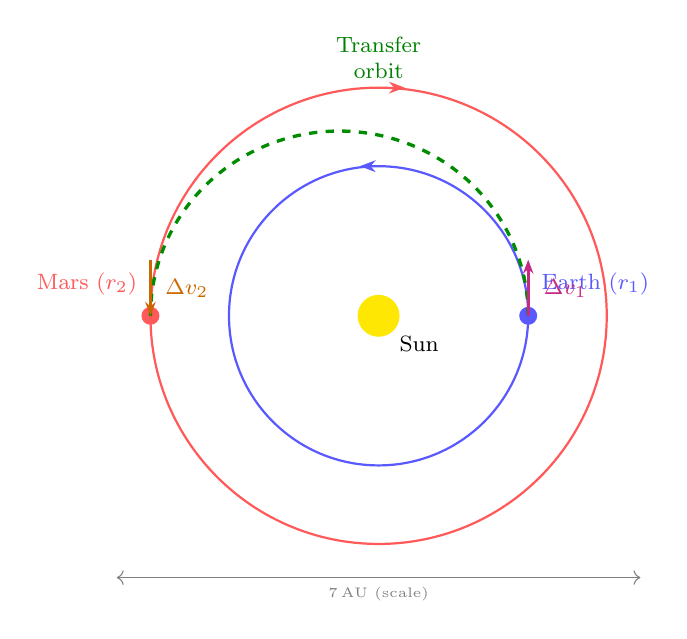
\begin{tikzpicture}[scale=0.95]
    % --- Sun ---
    \fill[yellow!90!orange] (0,0) circle (0.28cm);
    \node[below right, font=\footnotesize] at (0.15,-0.15) {Sun};
    % --- Earth orbit (r=2) ---
    \draw[blue!65, thick] (0,0) circle (2cm);
    \fill[blue!65] (2,0) circle (0.12cm);
    \node[above right, font=\footnotesize, blue!65] at (2.05,0.15) {Earth ($r_1$)};
    % --- Mars orbit (r=3.05) ---
    \draw[red!65, thick] (0,0) circle (3.05cm);
    \fill[red!65] (-3.05,0) circle (0.12cm);
    \node[above left, font=\footnotesize, red!65] at (-3.1,0.15) {Mars ($r_2$)};
    % --- Transfer ellipse upper half ---
    % Center at (-0.525,0), a=2.525, b=sqrt(6.1)~2.470
    \draw[green!55!black, very thick, dashed,
          domain=0:180, samples=120]
      plot ({-0.525 + 2.525*cos(\x)}, {2.470*sin(\x)});
    % --- Delta-v arrows ---
    \draw[-{Stealth[length=5pt]}, magenta!80!black, very thick]
      (2,0) -- (2,0.75);
    \node[right, font=\footnotesize, magenta!80!black] at (2.08,0.37)
      {$\Delta v_1$};
    \draw[-{Stealth[length=5pt]}, orange!80!black, very thick]
      (-3.05,0.75) -- (-3.05,0);
    \node[right, font=\footnotesize, orange!80!black] at (-2.98,0.37)
      {$\Delta v_2$};
    % --- Direction arrows ---
    \draw[-{Stealth}, blue!65, semithick] (0.05,2) -- (-0.25,2);
    \draw[-{Stealth}, red!65, semithick] (0.05,3.05) -- (0.35,3.05);
    % --- Label transfer ---
    \node[green!50!black, font=\footnotesize, align=center] at (0,3.45)
      {Transfer\\orbit};
    % --- Scale bar ---
    \draw[<->, gray, thin] (-3.5,-3.5) -- (3.5,-3.5)
      node[midway, below, font=\tiny] {$7\,\text{AU}$ (scale)};
  \end{tikzpicture}
  \caption{Hohmann transfer from Earth (blue, inner) to Mars (red, outer).
    The spacecraft receives impulse $\Delta v_1$ at Earth's orbit and, after
    \protect\SI{259}{\day}, is captured at Mars with braking impulse
    $\Delta v_2$. Orbit directions are shown by arrowheads.}
  \label{fig:hohmann}
\end{figure}

\subsection{Gravitational Assist Maneuvers}

A flyby of a massive planet can extract orbital energy from the planet and
transfer it to the spacecraft---at negligible cost to the planet. In the
planet's rest frame the spacecraft's speed is unchanged, but the direction
rotates through the \emph{deflection angle}
\begin{equation}
  \delta = 2\arcsin\!\left(\frac{1}{1 + r_p v_\infty^2/(GM_p)}\right),
  \label{eq:deflection}
\end{equation}
where $r_p$ is the periapsis distance and $v_\infty$ is the hyperbolic excess
speed. In the heliocentric frame, the speed change is
\begin{equation}
  \Delta v_\infty = 2v_p\sin\!\left(\frac{\delta}{2}\right),
  \label{eq:flyby}
\end{equation}
where $v_p$ is the planet's heliocentric speed. Voyager~2 used four successive
assists at Jupiter, Saturn, Uranus, and Neptune to achieve Solar System escape
velocity---a trajectory that would have required an additional
$\sim\SI{20}{\kilo\meter\per\second}$ of propellant using chemical engines alone.

\subsection{Low-Energy Transfers and the Interplanetary Superhighway}

Beyond Hohmann, \citet{Belbruno1987} demonstrated that the invariant manifolds
associated with libration points $L_1$ and $L_2$ of the Sun-Earth and
Sun-Moon three-body systems weave a network of low-energy pathways through
the Solar System. A transfer along these manifolds can reduce $\Delta v$
dramatically at the cost of increased transit time, exploiting the sensitive
dependence on initial conditions inherent in the three-body problem. The
governing equations are the Circular Restricted Three-Body equations:
\begin{align}
  \ddot{x} - 2\dot{y} &= x - \frac{(1-\mu)(x+\mu)}{r_1^3}
    - \frac{\mu(x-1+\mu)}{r_2^3}, \label{eq:cr3bp_x}\\
  \ddot{y} + 2\dot{x} &= y - \frac{(1-\mu)\,y}{r_1^3}
    - \frac{\mu\,y}{r_2^3}, \label{eq:cr3bp_y}
\end{align}
where $\mu = M_2/(M_1+M_2)$ is the mass parameter and $r_{1,2}$ are distances
from each primary. The Jacobi integral
\begin{equation}
  C_J = x^2 + y^2 + \frac{2(1-\mu)}{r_1} + \frac{2\mu}{r_2} - \dot{x}^2 - \dot{y}^2
  \label{eq:jacobi}
\end{equation}
is the single conserved quantity of the CR3BP and defines the \emph{zero-velocity
surfaces} that constrain possible trajectories.

% =============================================================================
\section[Advanced Propulsion: Beyond the Chemical Rocket]{Advanced Propulsion: Beyond the\\Chemical Rocket}
% =============================================================================

No chemical rocket can reach the stars. The Tsiolkovsky equation demands
impossible mass ratios for the required $\Delta v$. This section surveys the
propulsion technologies that may eventually make interstellar precursor
missions---and perhaps the stars themselves---reachable.

\subsection{Electric and Ion Propulsion}

Electric thrusters ionize a propellant (typically xenon) and accelerate the
ions electrostatically, achieving exhaust velocities far exceeding those of
chemical engines. The thrust--power relationship is
\begin{equation}
  F = \frac{2\eta_T\,P}{v_e},
  \label{eq:ion_thrust}
\end{equation}
where $P$ is input electrical power and $\eta_T$ is thruster efficiency
($\sim 0.6$--$0.7$). Because $v_e$ is large ($I_{\mathrm{sp}} \sim
\SI{3000}{}$--$\SI{10000}{\second}$), thrust is low but propellant
consumption is dramatically reduced. The Dawn mission used ion propulsion
to orbit both Vesta and Ceres---a dual-orbit mission impossible with chemical
propulsion.

\subsection{Solar Radiation Pressure and Photon Sails}

A photon sail uses solar radiation pressure. The radiation pressure on a
perfectly absorbing surface of area $A$ at heliocentric distance $d$ is
\begin{equation}
  P_\mathrm{rad} = \frac{L_\odot}{4\pi d^2 c}\quad \left(\frac{\text{N}}{\text{m}^2}\right),
  \label{eq:rad_press}
\end{equation}
where $L_\odot = \SI{3.828e26}{\watt}$ is the solar luminosity and $c$ is the
speed of light. For a perfectly reflecting sail of area $A$ and total system
mass $m$, the characteristic acceleration is
\begin{equation}
  a_{\mathrm{sail}} = \frac{2 L_\odot A}{4\pi d^2 m c}
    = \frac{L_\odot \sigma}{2\pi d^2 c},
  \label{eq:sail_acc}
\end{equation}
where $\sigma = A/m$ is the sail`s area-to-mass ratio. Contemporary
ultra-thin Mylar sails achieve $\sigma \sim \SI{100}{\meter\squared\per\kilo\gram}$.

\subsection{Nuclear Thermal Propulsion}

A nuclear thermal rocket heats propellant (hydrogen) in a reactor to
$\sim\SI{2700}{\kelvin}$, achieving $I_{\mathrm{sp}} \approx \SI{800}{}$--$\SI{1000}{\second}$
---roughly twice that of the best chemical engines. NERVA ground tests in the
1960s demonstrated this technology. The increased $I_{\mathrm{sp}}$ halves the
propellant mass required for a Mars transit.

\subsection{Nuclear Pulse Propulsion (Project Orion)}

Project Orion \citep{Dyson1968} proposed detonating nuclear bombs behind a
pusher plate to generate impulse. A series of $N$ explosions each providing
momentum $J_k = m_k v_k$ accelerates the spacecraft by
\begin{equation}
  \Delta v_{\mathrm{total}} = \eta_{\mathrm{plate}} \sum_{k=1}^N
    \frac{J_k}{M_k},
  \label{eq:orion}
\end{equation}
where $M_k$ is the spacecraft mass after the $k$-th explosion and
$\eta_{\mathrm{plate}}$ is the plate coupling efficiency. Theoretical
$I_{\mathrm{sp}}$ ranges from $10^4$ to $10^6$\,s, enabling a
crewed Saturn mission in weeks.

\subsection{Antimatter Propulsion}

Proton--antiproton annihilation releases the maximum possible energy per unit
mass:
\begin{equation}
  E = mc^2 \quad \Rightarrow \quad
  I_{\mathrm{sp,\,max}} = \frac{c}{g_0} \approx \SI{3.06e7}{\second}.
  \label{eq:antimatter_isp}
\end{equation}
For a mixed matter--antimatter propellant fraction $\phi$ (mass of
antimatter per total propellant mass), the effective exhaust velocity is
approximately
\begin{equation}
  v_e \approx c\sqrt{4\phi(1-\phi)},
  \label{eq:antimatter_ve}
\end{equation}
which peaks at $v_e = c$ for $\phi = 0.5$ (symmetric annihilation).
The principal barriers are production and storage: current antiproton
production yields $\sim \SI{1}{\nano\gram}$ per year at CERN, at a cost
of order $\num{e15}$\,USD per gram.

\subsection{Laser-Sail Propulsion (Breakthrough Starshot)}

For the smallest probes, a ground-based phased laser array of power $P_L$
can accelerate a photon sail of mass $m$ and reflectivity $R$ to
\begin{equation}
  a = \frac{(1+R)\,P_L}{mc},
  \label{eq:laser_accel}
\end{equation}
giving a final velocity (assuming acceleration over a distance $\ell$)
\begin{equation}
  v_f \approx \sqrt{\frac{2(1+R)\,P_L\,\ell}{mc}}.
\end{equation}
The Breakthrough Starshot initiative targets $v_f \approx 0.2c$ for a
\SI{1}{\gram} sail with $P_L = \SI{100}{\giga\watt}$, reaching Alpha
Centauri in about 20 years.

\begin{table}[ht]
  \centering
  \caption{Comparison of propulsion technologies.
           T.R.L.~=~Technology Readiness Level ($1$\,=\,basic principles,
           $9$\,=\,flight proven).}
  \label{tab:propulsion}
  \begin{tabularx}{\textwidth}{l r r c X}
    \toprule
    Technology & $I_{\mathrm{sp}}$ (s) & Thrust (N) & T.R.L. & Best use case \\
    \midrule
    Chemical (LOX/LH$_2$)  & 450            & $\sim\!10^6$ & 9 & LEO, interplanetary \\
    Kerosene/LOX           & 310            & $\sim\!10^7$ & 9 & Launch \\
    Ion (NSTAR)            & 3\,100         & $0.1$        & 9 & Deep space cruise \\
    Hall-effect (SPT-140)  & 1\,600         & 5.6          & 8 & GEO stationkeeping \\
    Solar sail             & N/A            & $10^{-3}$    & 5 & Near-Sun, small probes \\
    Nuclear thermal        & 900            & $\sim\!10^5$ & 4 & Mars, fast transits \\
    Nuclear pulse (Orion)  & $10^4$--$10^6$ & $\sim\!10^7$ & 2 & Outer SS, interstellar \\
    Fusion (D-T)           & $10^6$         & $10^3$       & 2 & Interstellar precursor \\
    Laser sail             & N/A            & variable     & 2 & Nano-probes to nearby stars \\
    Antimatter             & $\sim\!3\!\times\!10^7$ & variable & 1 & Full interstellar \\
    \bottomrule
  \end{tabularx}
\end{table}

% =============================================================================
\section{Relativistic Spaceflight}
% =============================================================================

\subsection{Special Relativity: A Brief Review}

At velocities approaching $c$, Newtonian mechanics fails. Einstein's special
relativity (1905) \citep{Einstein1905} introduces the Lorentz factor:
\begin{equation}
  \gamma \equiv \frac{1}{\sqrt{1-\beta^2}}, \qquad \beta \equiv v/c.
  \label{eq:gamma}
\end{equation}
Key consequences include time dilation ($\Delta t' = \gamma\,\Delta\tau$),
length contraction ($L = L_0/\gamma$), relativistic momentum
($\bm{p} = \gamma m\bm{v}$), and the energy--momentum relation:
\begin{equation}
  E^2 = (pc)^2 + (mc^2)^2.
  \label{eq:energy_momentum}
\end{equation}
Figure~\ref{fig:lorentz} shows the rapid growth of $\gamma$ as $\beta \to 1$.

\begin{figure}[ht]
  \centering
  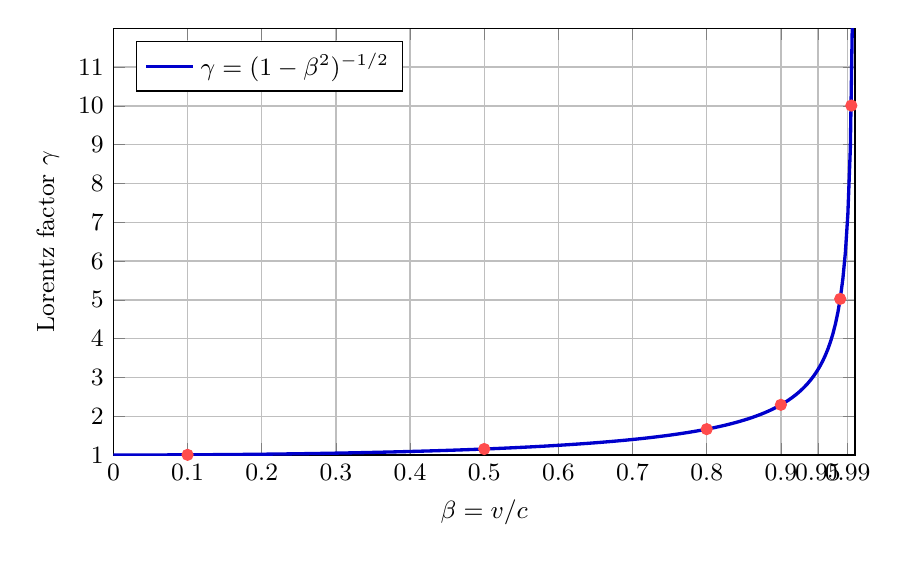
\begin{tikzpicture}
    \begin{axis}[
      width=11cm, height=7cm,
      xlabel={$\beta = v/c$},
      ylabel={Lorentz factor $\gamma$},
      xmin=0, xmax=1,
      ymin=1, ymax=12,
      xtick={0,0.1,0.2,0.3,0.4,0.5,0.6,0.7,0.8,0.9,0.95,0.99},
      xticklabels={0,0.1,0.2,0.3,0.4,0.5,0.6,0.7,0.8,0.9,0.95,0.99},
      ytick={1,2,3,4,5,6,7,8,9,10,11},
      grid=both,
      grid style={line width=0.3pt, draw=gray!25},
      major grid style={line width=0.5pt, draw=gray!50},
      tick label style={font=\small},
      label style={font=\small},
      legend pos=north west,
      legend style={font=\small},
    ]
      \addplot[blue!80!black, very thick, domain=0:0.997, samples=300]
        {1/sqrt(1-x*x)};
      \addlegendentry{$\gamma = (1-\beta^2)^{-1/2}$}
      % Mark a few reference points
      \addplot[only marks, mark=*, mark size=2pt, red!70]
        coordinates {(0.1, 1.005) (0.5, 1.155) (0.8, 1.667)
                     (0.9, 2.294) (0.98, 5.025) (0.995, 10.01)};
    \end{axis}
  \end{tikzpicture}
  \caption{Lorentz factor $\gamma$ as a function of $\beta = v/c$. Note the
    dramatic rise at $\beta \gtrsim 0.9$: at $\beta = 0.99$, an on-board clock
    runs more than 7 times slower than a stationary one.}
  \label{fig:lorentz}
\end{figure}

\subsection{The Relativistic Rocket Equation}

For a rocket with rest-frame exhaust velocity $v_e$, the relativistic
analogue of \eqref{eq:tsiolkovsky} is \citep{Ackeret1946}:
\begin{equation}
  \boxed{\frac{m_0}{m_f} = \left(\frac{1+\beta_f}{1-\beta_f}\right)^{c/(2v_e)},}
  \label{eq:rel_rocket}
\end{equation}
where $\beta_f = v_f/c$ is the final velocity fraction. Equivalently, using the
rapidity $\phi = \atanh(\beta)$:
\begin{equation}
  \frac{m_0}{m_f} = \exp\!\left(\frac{c}{v_e}\,\atanh(\beta_f)\right).
  \label{eq:rel_rocket_rap}
\end{equation}
For a perfect antimatter drive ($v_e = c$) and $\beta_f = 0.99$:
\begin{equation*}
  \frac{m_0}{m_f} = \exp\!\left(\atanh(0.99)\right) = \exp(2.65) \approx 14.
\end{equation*}
This is actually achievable---a factor of fourteen. For $\beta_f=0.999$
the ratio rises to $\sim 32$, still tractable for an advanced civilization.

\subsection{Constant-Acceleration Trajectories}

The most convenient mode of interstellar travel is constant proper acceleration
$a$ (the acceleration felt by passengers). The trajectory in a fixed inertial
frame is a \emph{Rindler hyperbola}:
\begin{align}
  x(\tau) &= \frac{c^2}{a}\!\left(\cosh\frac{a\tau}{c} - 1\right),
    \label{eq:rindler_x}\\
  t(\tau)  &= \frac{c}{a}\sinh\frac{a\tau}{c},
    \label{eq:rindler_t}\\
  v(\tau)  &= c\tanh\frac{a\tau}{c},
    \label{eq:rindler_v}
\end{align}
where $\tau$ is the traveller's proper time. The round-trip proper time to a
destination at coordinate distance $D$ (with phases: accelerate, decelerate,
accelerate back, decelerate to rest) is
\begin{equation}
  \tau_{\mathrm{RT}} = 4\,\frac{c}{a}\,\cosh^{-1}\!\!\left(\frac{aD}{2c^2}+1\right).
  \label{eq:rt_proper}
\end{equation}
For $a = g = \SI{9.81}{\meter\per\second\squared}$ (comfortable 1-\textit{g}
acceleration):

\begin{table}[ht]
  \centering
  \caption{Round-trip proper times for 1-$g$ continuous acceleration to selected
   destinations ($a=g$). Coordinate time $t_{\mathrm{RT}}$ is measured by a
   stationary observer; $\tau_{\mathrm{RT}}$ by the traveller.}
  \label{tab:rel_trips}
  \begin{tabularx}{\textwidth}{X r r r}
    \toprule
    Destination & $D$ & $t_{\mathrm{RT}}$ (coord.) & $\tau_{\mathrm{RT}}$ (proper) \\
    \midrule
    Mars (mean)           & \SI{0.52}{\AU}  & 63 days    & 63 days      \\
    Jupiter               & \SI{5.2}{\AU}   & 1.5 years  & 1.5 years    \\
    Pluto                 & \SI{39.5}{\AU}  & 4.4 years  & 4.3 years    \\
    Proxima Centauri      & \SI{4.24}{\ly}  & 5.9 years  & 3.5 years    \\
    Galactic Centre       & \SI{26000}{\ly} & 52\,026 years & 21.0 years\\
    Andromeda Galaxy      & \SI{2.5e6}{\ly} & 2.5 Myr    & 28.4 years   \\
    \bottomrule
  \end{tabularx}
\end{table}

The time dilation effect is profound: a crew travelling to Proxima Centauri
and back at 1~$g$ ages only 7 years, while 12 years pass on Earth. Travel
to the Galactic Centre ages the crew only 42 years---but 52\,000 years elapse
on Earth.

\subsection{Energy Requirements}

The kinetic energy imparted to the spacecraft (non-relativistic approximation
for $\beta \ll 1$) is $K = \half m_f \beta_f^2 c^2$. At relativistic
speeds, the total energy required is
\begin{equation}
  E_{\mathrm{kin}} = (\gamma_f - 1)\,m_f\,c^2.
  \label{eq:kinetic_rel}
\end{equation}
To accelerate a 1000-ton payload ($m_f = \SI{e6}{\kilo\gram}$) to $\beta=0.2$
requires
\begin{equation*}
  E = \left(\frac{1}{\sqrt{1-0.04}} - 1\right)\times \SI{e6}{}\times(\SI{3e8}{})^2
    \approx \SI{1.8e21}{\joule} \approx \SI{500}{\tera\watt\hour} \cdot
    \frac{1\,\mathrm{yr}}{8760\,\mathrm{h}},
\end{equation*}
comparable to roughly two months of total current global energy production.
Advanced fusion or antimatter reactors capable of sustained power outputs of
$10^{17}$--$10^{19}$\,W would be required---well within the range of a
Kardashev Type~II civilization (see Section~\ref{sec:kardashev}).

% =============================================================================
\section{The Population of Civilizations: A Statistical Argument}
\label{sec:civilizations}
% =============================================================================

\subsection{The Drake Equation}

How many technologically active civilizations currently exist in the Milky Way
capable of interstellar communication? Frank Drake \citep{Drake1961} proposed
the foundational estimate:
\begin{equation}
  \boxed{N = R_* \cdot f_p \cdot n_e \cdot f_l \cdot f_i \cdot f_c \cdot L,}
  \label{eq:drake}
\end{equation}
where:
\begin{itemize}[noitemsep]
  \item $R_*$: star formation rate in the Galaxy (yr$^{-1}$);
  \item $f_p$: fraction of stars with planetary systems;
  \item $n_e$: mean number of habitable-zone planets per planetary system;
  \item $f_l$: fraction of habitable planets on which life arises;
  \item $f_i$: fraction of life-bearing planets that develop intelligence;
  \item $f_c$: fraction of intelligent species that develop detectable
               technology;
  \item $L$: mean longevity of such a civilization (yr).
\end{itemize}

Table~\ref{tab:drake} summarises current estimates for each factor.

\begin{table}[ht]
  \centering
  \caption{Drake equation parameters: conservative, optimistic, and best-current
    estimates. The resulting $N$ spans more than 11 orders of magnitude.}
  \label{tab:drake}
  \begin{tabularx}{\textwidth}{X r r r}
    \toprule
    Parameter & Conservative & Optimistic & Best estimate \\
    \midrule
    $R_*$ (yr$^{-1}$) & 1    & 3          & 3    \\
    $f_p$              & 0.5  & 1.0        & 0.9  \\
    $n_e$              & 0.01 & 1.0        & 0.4  \\
    $f_l$              & $10^{-6}$ & 1.0  & 0.1  \\
    $f_i$              & $10^{-6}$ & 1.0  & 0.01 \\
    $f_c$              & 0.01 & 0.5        & 0.1  \\
    $L$ (yr)           & 100  & $10^9$     & $10^4$ \\
    \midrule
    $N$       & $\sim 10^{-10}$ & $\sim 10^8$ & $\sim 1200$ \\
    \bottomrule
  \end{tabularx}
\end{table}

\subsection{A Bayesian Reformulation}

\citet{Grinspoon2003} and others have advocated for treating the Drake parameters
as random variables with probability distributions. Let $\lambda_c$ be the
volumetric density of communicating civilizations. The probability that at
least one such civilization exists within an observable volume $V$---modeled
as a Poisson process---is:
\begin{equation}
  P(N \geq 1) = 1 - \ee^{-\lambda_c V}.
  \label{eq:poisson}
\end{equation}
If $N \sim \mathcal{N}(\mu_N, \sigma_N^2)$ in log-space (log-normal), the
expected value uses the arithmetic mean of the log-parameters. Crucially, the
Bayesian approach quantifies our uncertainty rather than hiding it behind
point estimates.

\subsection{The Fermi Paradox and Its Resolutions}

If $N$ is large, Fermi's question \citep{Hart1975} is unavoidable: \textit{``Where
is everybody?''} For $N \sim 10^6$, colonization of the Galaxy at modest
sub-light speeds ($\sim 0.01c$) should take $\sim 10^8$\,yr---a cosmic eye-blink
in a \SI{13.8}{Gyr}-old universe. Yet we observe no unambiguous signs of
extraterrestrial intelligence.

The principal resolutions cluster into three classes:
\begin{enumerate}[noitemsep]
  \item \textbf{Rarity.} Life or intelligence are extraordinarily rare (the
    \emph{Rare Earth} hypothesis \citep{WardBrownlee2000}); $N \ll 1$ always.
  \item \textbf{Filter.} There exists a ``Great Filter'' \citep{Hanson1998}:
    a low-probability transition that almost all evolutionary lineages fail.
    It may lie behind us (abiogenesis, eukaryogenesis) or ahead (technological
    self-destruction).
  \item \textbf{Communication.} Advanced civilizations exist but do not
    communicate in ways we have thought to look: the \emph{Zoo Hypothesis},
    the \emph{Dark Forest} \citep{Liu2008}, the \emph{Transcension Hypothesis}.
\end{enumerate}
The mathematical implication is sobering. If we detect no signal after a
thorough SETI survey (say, $10^9$ stars), then by Bayes' theorem we update
strongly toward $N \ll 1$ or toward the dark-forest scenario.

\subsection{The Kardashev Scale}
\label{sec:kardashev}

\citet{Kardashev1964} classified civilizations by their power consumption:
\begin{itemize}[noitemsep]
  \item \textbf{Type I:} uses all available power on its home planet,
    $P_{\mathrm{I}} \sim \SI{e16}{\watt}$.
  \item \textbf{Type II:} harnesses the full output of its star,
    $P_{\mathrm{II}} \sim \SI{4e26}{\watt}$ (solar luminosity).
  \item \textbf{Type III:} controls galactic-scale energy,
    $P_{\mathrm{III}} \sim \SI{e37}{\watt}$.
\end{itemize}
A continuous generalization \citep{Sagan1973} is:
\begin{equation}
  K = \frac{\log_{10} P_W - 6}{10},
  \label{eq:kardashev}
\end{equation}
where $P_W$ is total power in watts. Humanity in 2026 consumes roughly
\SI{2e13}{\watt}, giving $K \approx 0.73$---tantalizingly close to Type~I.

% =============================================================================
\section{Communication Across Interstellar Distances}
% =============================================================================

\subsection{Electromagnetic Communication}

All confirmed interstellar communication infrastructures are hypothetical, but
the physics is clear. A transmitter of power $P_t$ and gain $G_t$ (antenna
directionality) at distance $d$ delivers a signal power density at the
receiver of
\begin{equation}
  S = \frac{P_t\,G_t}{4\pi d^2}\quad (\text{W\,m}^{-2}).
  \label{eq:signal_density}
\end{equation}
The received power across collecting area $A_r = G_r\lambda^2/(4\pi)$ is
\begin{equation}
  P_r = P_t\,G_t\,G_r\!\left(\frac{\lambda}{4\pi d}\right)^2,
  \label{eq:friis}
\end{equation}
the Friis transmission equation. The signal-to-noise ratio in a bandwidth $B$
at system temperature $T_{\rm sys}$ is
\begin{equation}
  \mathrm{SNR} = \frac{P_t\,G_t\,A_r}{4\pi d^2\,\kB\,T_{\rm sys}\,B},
  \label{eq:snr}
\end{equation}
from which the minimum detectable flux density
$S_{\min} = \kB T_{\rm sys} B / A_r$ follows.

\subsection{The Cosmic Watering Hole}

\citet{Oliver1971} noted that the spectral interval between the hydrogen line
at $\nu_{\mathrm{HI}} = \SI{1420.4}{\mega\hertz}$ and the hydroxyl lines at
$\nu_{\mathrm{OH}} = \SI{1612}{}$--$\SI{1720}{\mega\hertz}$ is cosmically
quiet: local galactic synchrotron emission falls steeply, and the cosmic
microwave background noise floor is low. This ``watering hole'' defines a
natural gathering place for interstellar beacons. The Galactic centre in the
range 1--10\,GHz minimises the noise temperature contribution of the sum of
synchrotron, CMB, and atmospheric noise:
\begin{equation}
  T_{\rm noise}(\nu) \approx T_{\rm synchrotron}\,\nu^{-2.8}
    + T_{\rm CMB} + T_{\rm atm}(\nu).
\end{equation}
The minimum of $T_{\rm noise}$ occurs near \SI{2}{\giga\hertz}, motivating
SETI searches in this band.

\subsection{Channel Capacity and Numeric Estimates}

Shannon's channel capacity theorem \citep{Shannon1948} gives the maximum
information rate:
\begin{equation}
  C = B\log_2\!\left(1 + \mathrm{SNR}\right).
  \label{eq:shannon}
\end{equation}
For a transmitter of $P_t = \SI{10}{\tera\watt}$ (plausible Dyson-sphere
fraction), directed toward a $D = \SI{100}{\meter}$ telescope 10\,ly away,
with $B = \SI{1}{\hertz}$, $T_{\rm sys} = \SI{30}{\kelvin}$:
\begin{equation*}
  \mathrm{SNR} \approx \frac{10^{13} \times 10^8 \times 7854}{4\pi (10^{17.5})^2
    \times 1.38\times 10^{-23} \times 30 \times 1} \approx 3\times 10^{3}.
\end{equation*}
A \SI{10}{\tera\watt} beacon 10\,ly away is easily detectable with a
100-m dish---if we know where and at what frequency to look.

For laser communication in the optical/near-infrared, pulsed lasers with
peak powers of $P_\ell = \SI{100}{\tera\watt}$ (achievable with nanosecond
pulse duration) would outshine the Sun by several orders of magnitude in the
visible band during the pulse, providing an unambiguous technosignature.

% =============================================================================
\section{A Universal Language for First Contact}
% =============================================================================

\subsection{Mathematical Universals}

Any sufficiently advanced civilization must have discovered the same
mathematical truths: the primality of 2, 3, 5, 7, 11; the value of $\pi$;
the structure of Euclidean geometry; and the physical constants of nature.
Mathematics is not a human invention but a discovery of patterns inherent in
physical reality---a view sometimes called \emph{mathematical Platonism}
\citep{Penrose1989}. It is the only framework guaranteed to be interpretable
by any intelligence that has mastered technology.

\subsection{The Lincos Proposal and Prime-Number Encoding}

Hans Freudenthal's \emph{Lingua Cosmica} (Lincos, 1960) \citep{Freudenthal1960}
proposed building an interstellar language from scratch. The encoding
hierarchy is:
\begin{enumerate}[noitemsep]
  \item \textbf{Numbers.} An unambiguous encoding of natural numbers (e.g., burst
    counts: 2 pulses, 3 pulses, 5 pulses, 7 pulses, 11 pulses, \ldots, all prime)
    establishes that the signal is artificial.
  \item \textbf{Arithmetic.} Sequences such as $2 + 3 = 5$ in burst form teach
    the arithmetic operators.
  \item \textbf{Logic.} The Boolean constants and propositional operators.
  \item \textbf{Relations.} Equality, ordering, set membership.
  \item \textbf{Physical referents.} Using the message itself to transmit
    units of time (period of the carrier) and space (its wavelength), and then
    encoding mass via the hydrogen mass \mbox{$m_H = \SI{1.67e-27}{\kilo\gram}$}.
\end{enumerate}

The dimensionless constants of nature---the fine-structure constant
$\alpha$, the proton-to-electron mass ratio $\mu$---are universal signatures:
\begin{equation}
  \alpha = \frac{e^2}{4\pi\varepsilon_0\,\hbar c} \approx \frac{1}{137.036},
  \qquad
  \mu = \frac{m_p}{m_e} \approx 1836.15.
  \label{eq:constants}
\end{equation}
Encoding these values serves as a ``password'' proving that the sender
shares the same physics.

\subsection{Two-Dimensional Pixel Encoding}

Mapping a total bit count $N = p \times q$ (where $p$, $q$ are distinct primes)
into a 2D grid of size $p \times q$ allows the receiver to reconstruct an image
by the unique factorization into primes. The 1974 Arecibo message used exactly
this technique: $1679 = 73 \times 23$ bits, encoding a $73 \times 23$ pixel image
containing the solar system, DNA structure, and a human figure.

If the message length is $N = p_1 \times p_2 \times p_3$ (three distinct primes),
a three-dimensional data structure is implied---a powerful extension for
transmitting sequences of images or mathematical tables.

% =============================================================================
\section{Establishing Interstellar Relations: Diplomacy Across the Void}
% =============================================================================

\subsection{Game Theory of First Contact}

The contact problem can be modeled as a coordination game. Let civilization A
and civilization B each choose strategy $s \in \{S, \varnothing\}$ (Signal or
Silence). The payoff matrix (row = A's strategy, column = B's) is:

\begin{equation}
\begin{pmatrix}
  & S & \varnothing \\
  S & (b-c,\; b-c) & (-c,\; b) \\
  \varnothing & (b,\; -c) & (0,\; 0)
\end{pmatrix}
\label{eq:payoff}
\end{equation}
where $b > 0$ is the benefit of mutual contact and $c > 0$ is the cost of
transmitting. If $b > c$, mutual signaling $(S, S)$ is a \emph{Nash
equilibrium}; neither party has a unilateral incentive to deviate. The ``Dark
Forest'' scenario \citep{Liu2008} posits $b < 0$ (contact is dangerous),
which yields \emph{Silence} as the dominant strategy for both---an
interpretation of the Fermi paradox consistent with game theory.

\subsection{The Prisoners' Dilemma and Iterated Contact}

A single interaction offers limited cooperation incentives. However,
interstellar contact is necessarily iterated: even at light-speed, an exchange
with a civilization 40\,ly away takes 80 years per round-trip. \citet{Axelrod1984}
showed that in iterated prisoners' dilemma games, the strategy
\emph{tit-for-tat} (cooperate on round 1, then mirror the partner's previous
move) is remarkably robust. The expected payoff over $T$ rounds is:
\begin{equation}
  U(T) = b + (T-1)\left[b\,p_{\rm coop} - c\,p_{\rm defect}\right],
  \label{eq:iterated}
\end{equation}
where $p_{\rm coop}$ and $p_{\rm defect}$ are the cooperation and defection
probabilities. For long-lived civilizations ($T \gg 1$), cooperation dominates
if $b > c$.

\subsection{Protocols Inspired by Diplomacy}

Any civilized contact regime should incorporate:
\begin{itemize}[noitemsep]
  \item \textbf{Declaration of intent.} The first message establishes benign
    purpose, mathematical in nature: the transmission of physical constants and
    mathematical theorems verifiable by any intelligence.
  \item \textbf{Information asymmetry.} A richer party should be prepared to
    give more information initially to establish trust.
  \item \textbf{Temporal patience.} Given light-speed delays of decades to
    millennia, political structures on both ends will change between message and
    reply. Institutions---not individuals---must maintain the correspondence.
  \item \textbf{Non-directional broadcasting.} For unknown civilizations,
    broadcasts should be omnidirectional (or cover wide galactic segments) using
    narrowband carriers near the ``watering hole.''
\end{itemize}

\subsection{The Ethics of Contact}

What obligations arise if we detect an extraterrestrial signal? Three ethical
frameworks yield different answers:
\begin{itemize}[noitemsep]
  \item \textbf{Utilitarian:} If the expected information gain is enormous and
    the risk manageable, aggressive response is justified.
  \item \textbf{Precautionary:} The potential existential risk of revealing our
    location to an unknown civilization counsels silence (the Dark Forest
    argument made prescriptive).
  \item \textbf{Cosmopolitan:} All intelligent beings share a moral community;
    non-response is a form of isolationist parochialism.
\end{itemize}
At present, the IAA SETI Committee recommends a receive-only policy pending
international consensus on reply protocols---a cautious but defensible position
in the absence of information about the Other.

% =============================================================================
\section{Toward a Galactic Civilization}
% =============================================================================

\subsection{Information, Energy, and Complexity}

A fundamental insight of modern physics is that \emph{information is physical}
(Landauer's principle):
\begin{equation}
  \Delta Q_{\min} \geq \kB T \ln 2 \approx \SI{2.87e-21}{\joule}
  \quad (T = \SI{300}{\kelvin}),
  \label{eq:landauer}
\end{equation}
the minimum heat dissipated per erased bit. Computational complexity is bounded
by the available free energy. A civilization's information-processing capacity
scales with its energy budget: the transition from Kardashev~I to II to III
corresponds to jumps of $\sim 10^{10}$ in computational capacity.

\subsection{Civilizational Trajectories}

If civilizations reliably reach Type~II ($\sim\!10$ billion years of stellar
evolution available), the Galaxy has had time to be colonized several times
over. The observation that it has not---or appears not to have been---is either
the strongest evidence for the Great Filter ahead, or an indication that
expanding civilizations converge to stable, low-footprint configurations
(the \emph{Transcension Hypothesis}: advanced intelligence moves inward, toward
increasing complexity and miniaturization, rather than outward toward territorial
expansion).

\subsection{The Long View: Humanity's Place in the Cosmic Web}

On cosmological timescales the universe is young. The \emph{stelliferous era}
will last~$\sim\!10^{14}$\,yr; red and brown dwarf stars will support
habitable planets long after the Sun has become a white dwarf. A civilization
that survives the coming millennia will find itself in a universe that, by
current stellar formation rates, has not yet reached half its total
star-forming lifetime. The moral weight of the long future---the potential
beings who could exist if civilization endures---is an overwhelming argument
for treating the expansion of life into the cosmos as a civilizational
priority of the highest order.

% =============================================================================
\section{Conclusions}
% =============================================================================

We have traced a continuous mathematical thread from the vis-viva equation of
planetary motion to Shannon's channel capacity theorem applied to interstellar
beacons---a thread connecting orbital mechanics, rocket thermodynamics, the
geometry of spacetime, and the information theory of language.

The analysis yields firm conclusions:
\begin{enumerate}[noitemsep]
  \item Chemical propulsion is categorically incapable of interstellar flight;
    fusion or antimatter drives, or laser propulsion for small probes, are the
    minimum required.
  \item Relativistic travel to the nearest stars is physically possible within
    a human lifetime on board, but requires energy budgets orders of magnitude
    beyond current civilization---reachable, though, by a Kardashev Type~I or
    Type~II civilization.
  \item The Drake equation is consistent with both $N \gg 1$ and $N \approx 0$;
    current data cannot resolve the ambiguity, but future biosignature surveys
    (JWST, Habitable Worlds Observatory) will dramatically narrow the range.
  \item Electromagnetic communication at gigawatt-to-terawatt power levels is
    fully detectable across tens of light-years with near-future radio and
    optical telescopes; the principal barrier is pointing, frequency, and time.
  \item Mathematics provides the only culturally neutral language for first
    contact; prime numbers, universal constants, and geometric encodings are the
    universal foundation.
  \item Game theory favors interstellar cooperation when civilizational lifetimes
    are long and contact is iterated; the long-term expected value of mutual
    communication is positive for most realistic parameter choices.
\end{enumerate}

The stars are not infinitely distant. They are separated from us by time,
energy, and courage---all three of which humanity has shown, in its brief
cosmic history, that it possesses in abundance. The question is not \emph{if}
we will reach them, but \emph{when}, and \emph{who we will meet} when we do.

% =============================================================================
% APPENDICES
% =============================================================================
\appendix

\section{Derivation of the Relativistic Rocket Equation}
\label{app:rel_rocket}

Consider a rocket of instantaneous mass $m$ and velocity $\beta c$ emitting
a photon (or relativistic exhaust) of infinitesimal energy $\dd E = (- \dd m)\,
v_e$ in the rocket rest frame. In the lab frame, 4-momentum conservation gives
\begin{equation}
  \frac{\dd(\gamma\beta)}{-\dd m/m} = \frac{v_e/c}{1 - v_e\beta/c^2},
\end{equation}
which upon integration yields (for constant $v_e$)
\begin{equation}
  \int_0^{\beta_f} \frac{c\,\dd\beta'}{(1-\beta'^2)(1 - v_e\beta'/c^2)}
  = -v_e \ln\frac{m_f}{m_0}.
\end{equation}
For $v_e = c$ (photon drive) the integral evaluates to $c\,\atanh(\beta_f)$,
leading directly to equation~\eqref{eq:rel_rocket_rap}.

\section{Numerical Values of Key Physical Constants}
\label{app:constants}

\begin{tabular}{ll}
  \toprule
  Constant & Value \\
  \midrule
  Speed of light & $c = \SI{2.998e8}{\meter\per\second}$ \\
  Gravitational constant & $G = \SI{6.674e-11}{\meter\cubed\per\kilo\gram\per\second\squared}$ \\
  Boltzmann constant & $\kB = \SI{1.381e-23}{\joule\per\kelvin}$ \\
  Solar mass & $\Msun = \SI{1.989e30}{\kilo\gram}$ \\
  Solar luminosity & $L_\odot = \SI{3.828e26}{\watt}$ \\
  Astronomical unit & $\SI{1}{\AU} = \SI{1.496e11}{\meter}$ \\
  Light-year & $\SI{1}{\ly} = \SI{9.461e15}{\meter}$ \\
  Hubble constant & $H_0 = 67.4$\,km\,s$^{-1}$\,Mpc$^{-1}$ \\
  \bottomrule
\end{tabular}

% =============================================================================
% BIBLIOGRAPHY
% =============================================================================
\bibliographystyle{plainnat}
\bibliography{references}

\end{document}
